%!TEX root = volumeFinal.tex 

\chapter{\label{chap:impl}Projeto de Implementação}

\begin{itemize}
	\item blablabla inicial- ver ramon
	\item JSHOP2
	\item MicroRTS -arquitetura-abstraction-tecnicas presente
	\item Modelagem do dominio
	\item heuristica
	\item implementação - como foi colocar o jshop dentro do java, tradução do problema na mão, algoritmo e modificações
\end{itemize}



\begin{itemize}
	\item - Modelagem - Jogo - HTN
	\item - Heuristica
	\item - Implementação e experimentos
\end{itemize}






\subsection{Arquitetura do MicroRTS}

A arquitetura do MicroRTS é composta por 3 componentes principais. São eles:

\begin{itemize}
	\item Logica do jogo, é onde todas as ações do jogo são validadas e interpretadas;
	\item Unidades, é onde todas as unidades são acessadas; e
	\item Interface gráfica, é onde todas as informações da logica do jogo e das unidades é apresentada de forma gráfica.
\end{itemize}

O MicroRTS permite que seja acoplado facilmente técnicas de IA. A IA deve obter informações do jogo através da logica do jogo e das unidades, e ter um método para geração das ações. A imagem \ref{fig:pacotes} representa os componentes e como eles devem se comunicam.

\begin{figure}[ht]
	\centering
	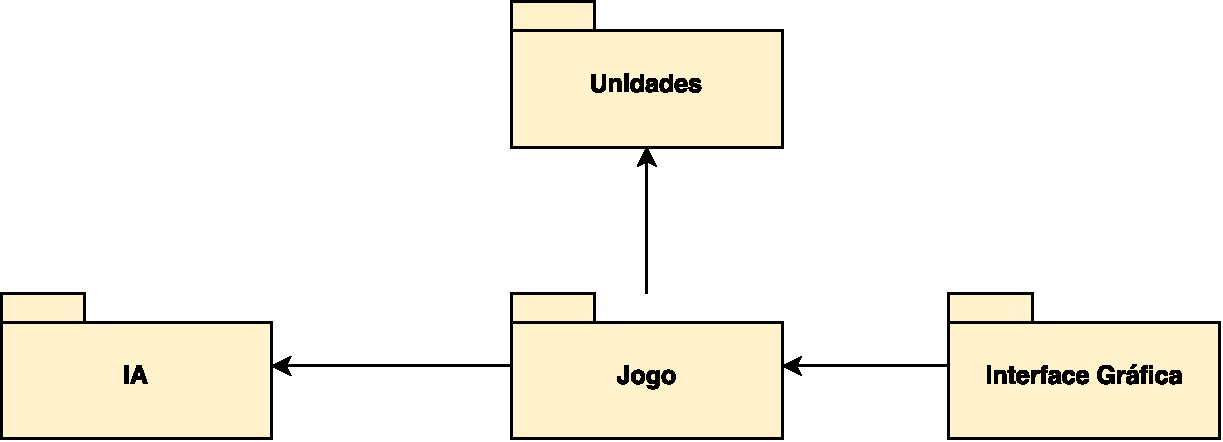
\includegraphics[width=0.4\textwidth]{fig/pacotes.pdf}
	\caption{Arquitetura MicroRTS}
	\label{fig:pacotes}
\end{figure}

O MicroRTS conta com cinco classes principais para funcionamento do jogo e uma para controle da IA. O diagrama de classes presente na Figura~\ref{fig:classes} ilustra os principais métodos das classes originadas do MicroRTS. As funcionalidades de cada classe encontra-se à seguir: 

\begin{itemize}
	\item \textit{GameVisualSimulation} é a interface entre os componentes do jogo e o usuário;
	\item \textit{GameState} e \textit{PhysicalGameState} são responsáveis pelo controle das ações das unidades dentro do mapa;
	\item \textit{UnitTypeTable} é onde cada unidade está associada as ações possíveis no jogo;
	\item \textit{PhysicalGameStatePanel} é responsável pela interface gráfica; e
	\item \textit{IA} é onde a técnica de IA deve ser acoplada ao jogo.
\end{itemize}

\begin{figure}[ht]
	\centering
	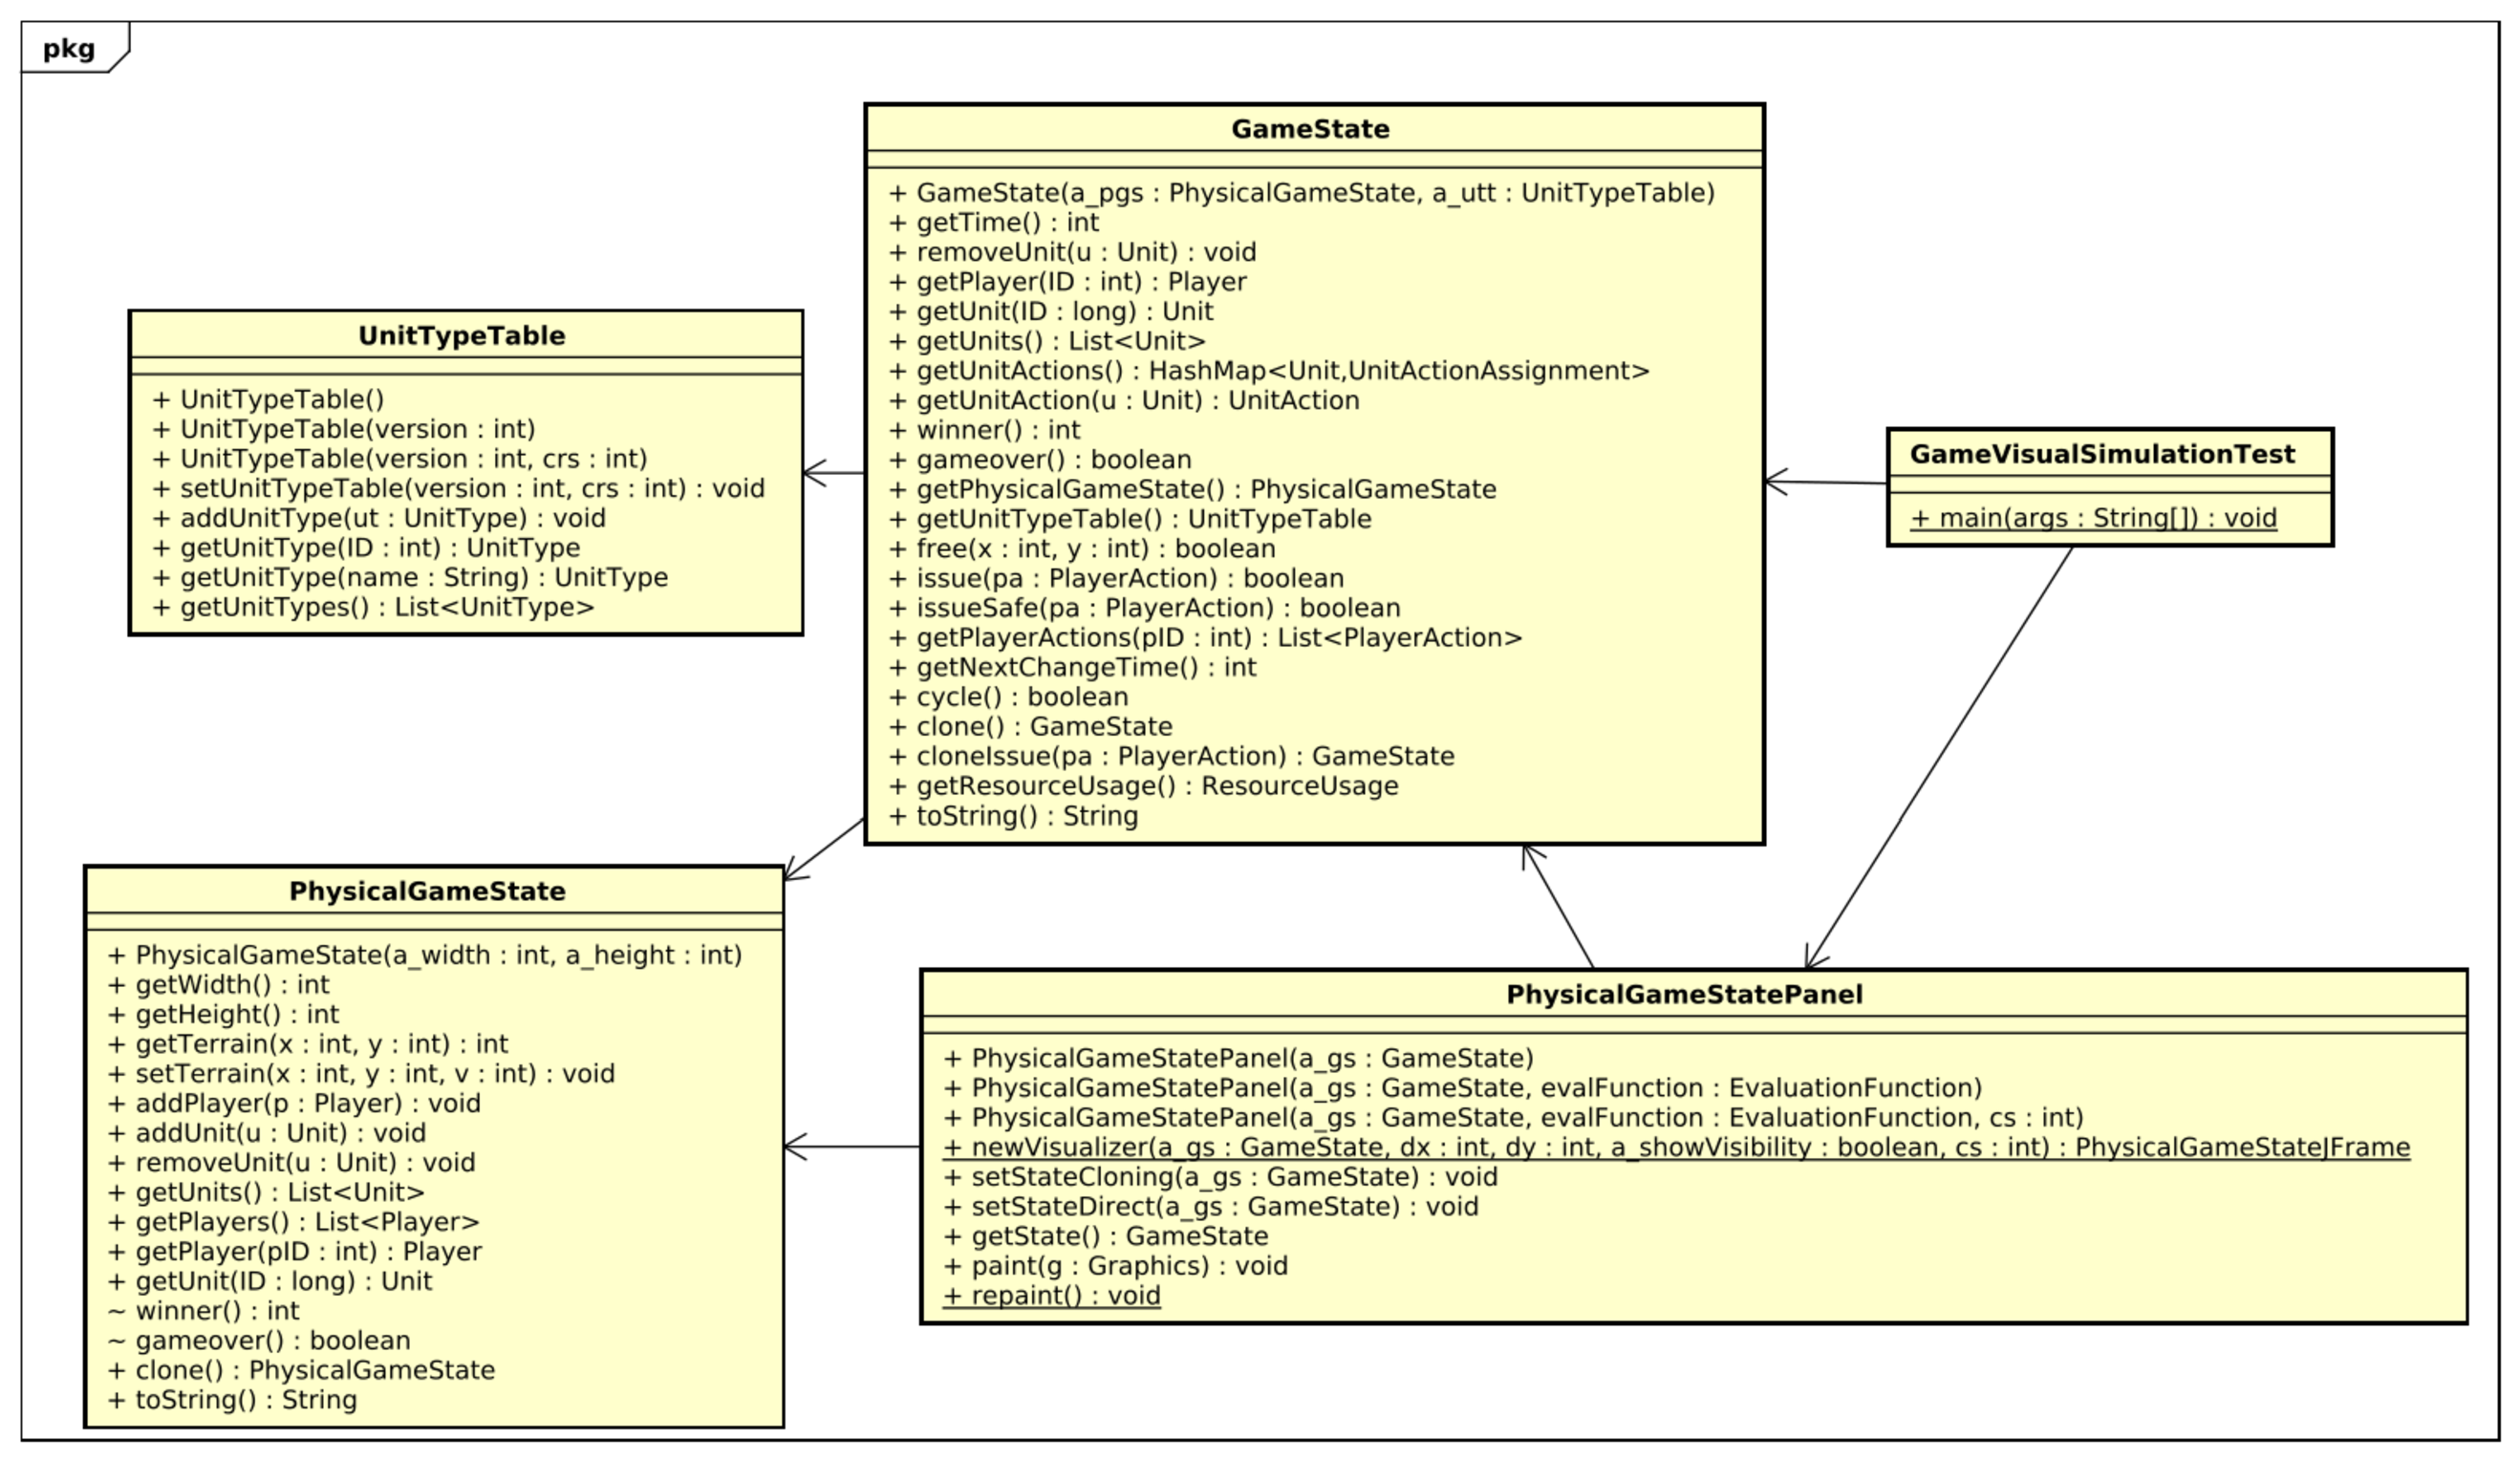
\includegraphics[width=1\textwidth]{fig/classes.pdf}
	\caption{Classes do MicroRTS}
	\label{fig:classes}
\end{figure} 

\subsection{Técnicas de IA}